
\begin{abstract}

A diabetes diagnosis entails important consequences for its recipients. Diagnosed patients obtain health information but also face the challenge of having to manage the condition via lifestyle adjustments, with potential consequences for---among other things---their economic activity. We investigate the causal effect of a diabetes diagnosis on employment status and behavioural risk-factors, two potentially intertwined factors, using longitudinal data from the \acf{CHNS} that cover the years 1997 to 2011. Two complementary statistical techniques---marginal structural models and fixed effects panel estimation---are used for the statistical analysis, and generate very similar results despite their different underlying assumptions. Both strategies find distinct patterns for males and females. They suggest a decrease in female employment probabilities after a diagnosis (over 11 percentage points) and further show that women are mostly unable to positively change their behavioural risk factors by loosing weight and reducing energy intake. Men, however, do not see their employment probabilities affected by diabetes and also respond to a diagnosis by losing weight and reducing energy intake as well as their intake of alcohol in ways that are sustained over time. These results suggest important inequities in the impact of diabetes between sexes in China and point to the potential of reducing behavioural risk factors for women to narrow these inequities.


\end{abstract}


\section{\label{sec:Introduction5}Introduction}

The effect of diabetes on employment status has received relatively little attention in \acp{MIC}, including China. The scarce existing evidence indicates that diabetes can affect labour market outcomes in \acp{HIC}, but also in \acp{MIC} \parencite{Seuring2016}. This is of growing relevance especially with diabetes appearing increasingly earlier in a person's productive lifespan, among others due to increasing obesity at earlier ages. Importantly, once diagnosed, the onset of diabetes, and diabetes complications, strongly depend on the patient's behaviour. Behavioural risk factors like alcohol consumption, smoking, caloric consumption and weight gain are all related to the onset of diabetes as well as ensuing diabetes complications. Research shows for instance that behaviour changes after a diabetes diagnosis can have positive health effects and reduce the risk of subsequent cardiovascular events \parencite{Long2014} and may help in effectively managing blood glucose levels and achieving further treatment goals \parencite{Zhou2016}. Consequently, if these risk factors can be reduced it may be possible to prevent some of the health and economic burden of diabetes. Thus, it seems that a diabetes diagnosis may present an important opportunity to reduce risk factors for diabetes complications \parencite{DeFineOlivarius2015} and hence also reduce the economic burden of diabetes to the individual. This raises the question how diabetes diagnosis affects both labour market outcomes and health behaviour over time.

However, one of the challenges of determining a causal relationship between  diabetes, employment status and changes in behavioural risk factors is their potential bidirectional interrelatedness. For example, employment status might by affecting weight status by reducing the time spend on physical activity due to reductions in available leisure time, or it may promote risk factors such as smoking behaviour or energy intake that can both affect the probability of developing diabetes as well as diabetes related complications, for instance by increasing stress levels. In an effort to  investigate the dynamic impact of unemployment on health behaviours, \textcite{Colman2014} found heterogeneous effects of unemployment which led to slight weight gain, a decrease in smoking and decreases in fast-food consumption. Macroeconomic evidence also indicates that job loss can lead to changes in health, especially in mental health \parencite{Charles2008}, which may have further downstream effects on health behaviours.

Research on the impact of diabetes on labour market outcomes has so far ignored the potentially simultaneous relationship of diabetes with employment and behavioural diabetes risk factors. Using regression techniques such as \ac{OLS} or \ac{FE} it was assumed that the investigated independent variables are unaffected by prior values of the dependent variable. However, if prior changes in employment status are causally related to a diabetes diagnosis or affect the risk factors for diabetes complications, not accounting for this can lead to biased estimates.\footnote{One solution is to include lagged values of the dependent variable on the right hand side, but this raises challenges of its own, including difficulty of interpretation, but also potentially biased estimates. The lagged dependent variable will be correlated with the time-invariant part of the error-term, violating the assumption of exogeneity of the right-hand side variables. Further, if the other covariates are correlated with the lagged-dependent variable, they will also be biased \parencite{Anderson1982,Nickell1981}.} Similarly, studies investigating the impact of a diabetes diagnosis on behavioural risk factors while not taking into account the effect of employment status on both diabetes and these risk factors, may produce biased estimates. Moreover, apart from time-varying confounding due to observed covariates, unobserved variables present a further challenge. In particular, time-invariant confounders---such as poor early life conditions or personal trades---may simultaneously increase the probabilities to develop diabetes, to be unemployed and to engage in unhealthy behaviour. 

The goal of this study is therefore to assess the impact of a diabetes diagnosis on both employment probabilities and behavioural risk factors while accounting for the potentially intertwined relationships between diabetes, employment and health behaviours. This is done via the use of \acp{MSM}, an estimation strategy that is increasingly common in epidemiology and is able to account for time-dependent confounding across time \parencite{Robins2000} when estimating the impact of a treatment, here a diabetes diagnosis, on the outcome of interest. This is, by our knowledge, the first time this estimation strategy is used to estimate the impact of diabetes on an individual's employment status or behavioural risk factors. We complement this strategy and test the robustness of the \ac{MSM} estimates to the potential violation of one of its crucial assumptions, namely that there are no unmeasured confounding factors. To do this, we compare them with \ac{FE} models which, although unable to account for the potentially bidirectional relationship, do account for unobserved time-invariant confounding factors in addition to confounding due to observed variables. Very different results to the \ac{MSM} would suggest a violation of the assumption of no unobserved confounding. To further investigate and understand the role of confounding factors, we also estimate \ac{RE} models and compare the results.  We thereby further extends the evidence base for the impact of diabetes on labour market outcomes in \acp{MIC}, where currently empirical information is only available for Mexico \parencite{Seuring2016}. At the same time the study provides, as far as we are aware, the first longitudinal evidence for the effect of a diabetes diagnosis on behavioural risk factors in any \acp{LMIC}  country.

 
More information about the effects of a diabetes diagnosis may be particularly important for \acp{LMIC} such as China, where diabetes prevalence has surged from 1\% in the early 1980s to about 10\% in recent years \autocite{Hu2011,Risk2016}. Confronting this diabetes epidemic puts a strain on healthcare systems \parencite{Seuring2015a}, increasing the need to find highly cost-effective prevention and treatment options applicable in \acp{MIC} \parencite{WHOresearchpriorities2010}. However, to do this it is important to assess how successful people with diabetes currently are in preventing adverse economic effects and reducing their risk factors for diabetes complications.


%Finally, another study on China also used diabetes biomarkers to identify those formally unaware of their diabetes, assuming that they were informed about their diabetes status by the survey team \parencite{Liu2014}. They use a difference in difference approach to identify the effect of a diagnosis on labour income in the wave after diagnosis, finding a decrease of about 16\%. They attribute this effect to the psychological consequences of the diabetes diagnosis, however, they are not able to rule out an effect of a deterioration of health on income. Further, the results only provide a short term picture, and it remains unclear if people are able to recover from the initial shock. ONLY INCLUDE IF I ALSO LOOK AT INCOME


The literature trying to identify a causal relationship between diabetes and employment has relied on \ac{IV} strategies \parencite{Brown2005,Latif2009,Seuring2015} and individual \ac{FE} models \parencite{Seuring2016}. However, while an \ac{IV} approach could potentially account for all forms of confounding, the validity of the instruments used is at least questionable (see discussion in Chapter \ref{cha:Mex2}). The \ac{FE} model, as discussed above, also relies on important assumptions that may be violated. Turning to the relationship between a diabetes diagnosis and behavioural risk factors, only one study has intended to causally relate a recent diabetes diagnosis with changes in health behaviours, finding positive behaviour changes shortly after diagnosis in a USA population. The found effects were mostly short lived and tended to dissipate over time, particularly considering weight loss \parencite{Slade2012}. To isolate the causal effect \textcite{Slade2012} created an 'at risk' control group without diabetes that was intended to be similar to the treatment group with diabetes, apart from not having received a diagnosis. He used information on diabetes biomarkers to estimate the propensity score of those without a diabetes diagnosis to be above a specific at risk threshold, so that everybody above a certain propensity score was used to form the control group. He then estimated dynamic population average models, including the lagged dependent variable on the right hand side, as well as \ac{FE} models to identify a causal relationship. While this approach likely improves the control group by increasing its similarity in the diabetes risk profile to the diagnosed population, the use of a lagged dependent variable may have biased the estimates due to unobserved time-invariant variables being correlated with the lagged dependent variable, violating the exogeneity assumption and potentially introducing bias in the other covariates. This is also true for the \ac{FE} model \parencite{Nickell1981,Anderson1982}. Further, the study did not account for employment status as one of the control variables. 

A different identification approach was used by \textcite{Zhao2013a} when investigating the effects of a hypertension diagnosis on nutritional outcomes in China. They used a regression-discontinuity design and biomarker information on blood pressure. A crucial assumption in that study was that people above the hypertension threshold were indeed informed about their hypertension while those just below the threshold were not. These two groups were then compared to isolate the particular effect of the additional health information on food consumption in the following wave. The results indicated that a diagnosis leads to reductions in fat consumption, but no other nutritional outcomes, and only for those economically better off. Several caveats exist for this study and the used approach. According to \textcite{Zhao2013a}, it was not always clear to what extent participants were informed about their hypertension status and whether they had received just the actual blood pressure measurement information, leaving the interpretation to the participants, or whether they were made explicitly aware of their hypertension (or also pre-hypertension) status. Further, the results may have limited generalisability, since the measured treatment effect may have been a very local one, depending on the representativeness of the population distribution below and above the threshold of the overall population above the threshold. In the case of significant differences between the populations, the results would only be applicable to the population around the hypertension threshold. Finally, the study only provides information for a relatively short period until the first wave after diagnosis, unable to capture any changes further away from the point of diagnosis. 

Accordingly, there is a need to provide new evidence on the effects of a diabetes diagnosis on employment status as well as behavioural risk behaviours that could affect the development of diabetes complications, using longitudinal data and alternative estimation strategies. Thereby this study adds in several ways to the existing literature. First, it shows the impact of diabetes diagnosis on labour market outcomes in China, not only over the short term, but for a period covering the entire decade of the 2000s, allowing for a more long term investigation of the effects. This both confirms and extends earlier evidence for other settings and using different methods. Second, it provides information on the effect of a diabetes diagnosis on health behaviours. Third, by considering the effects over time on both employment and health behaviour, the results shed light on potential pathways through which the impact on employment may work.  Fourth, the study provides a methodological innovation by using both \ac{MSM} and \ac{FE} estimation methods, offering insights not only on the robustness of the \ac{MSM} results, but also on the validity of some of its assumptions.  


\section{\label{sec:Methods5}Methods}

\subsection{Study sample}


The \acf{CHNS} is an international collaborative project, led by the Carolina Population Center at the University of North Carolina at Chapel Hill, investigating nutrition and health behaviours in nine provinces of China \parencite{Zhang2014d}. We use data from 1997 onwards, which was the first time survey participants provided diabetes information. In total we use six waves (1997, 2000, 2004, 2006, 2009 and 2011) obtained from the longitudinal dataset released in 2015. The data provide extensive information on nutrition and health. Importantly this includes anthropometric measures of weight and height that reduce potential measurement issues plaguing self-reported data. It further provides socioeconomic information, most importantly for this study about employment. The sample is limited to the adult population aged 18--64.  The sample is not nationally representative and as such does not provide sampling weights  \parencite{Popkin2010}.

Overall, between 84\% to 90\% of the survey participants were followed up in the consecutive wave, with attrition being highest after 2006. Attrition in the \ac{CHNS} due to mortality was around 1\% \parencite{Popkin2010}. Other reasons mentioned by \textcite{Popkin2010} are loss in follow up due to migration, natural disasters and redevelopment of housing in the urban centres leading to relocations. We investigated whether any of our variables of interest was significantly related to attrition at any wave. Lower calorie consumption and being unemployed were associated with attrition. Further, attrition was strongly related to urbanization, a higher level of education, being of younger age and having lower family income, suggesting that mostly participants of younger age, more urbanized but from less well-off households tended to leave the survey. Having diabetes was not related to attrition. Attrition rates between the waves are shown in Table \ref{tab:attrition} in the appendix.


\subsection{Assessment of diabetes}

We used self-reported information on a diabetes diagnosis to construct our diabetes indicator. We only relied on incident cases of self-reported diabetes, excluding individuals with self-reported diabetes at baseline. Given the chronic nature of diabetes, we assumed that after the initial diagnosis diabetes persists for the rest of one's life. This is a reasonable assumption given the medical evidence \parencite{Steven2016}.\footnote{Recently, a study showed successful remission of at least 6 months in some patients after the initiation of a very low-calorie diet \parencite{Steven2016}. However, while this shows that type 2 diabetes may be reversible, this cannot be expected for patients diagnosed and currently treated in any healthcare system.} To construct a measure of diabetes duration for incident cases we used self-reported information on the year of diagnosis. If we found that the year of diagnosis was reported to be before the last wave without a reported diagnosis or if the year of diagnosis was not reported, we used the midpoint between the last wave without diagnosis and the first wave with a diagnosis as the year of diagnosis.\footnote{The number of observations replaced at each wave was: 21 (2000), 44 (2004), 51  (2006), 78 (2009), 59 (2011). Overall it affected 43\% of the self-reports of the year of diagnosis.}

\subsection{Assessment of outcomes}

The economic outcome of interest is employment status, and is measured through self-reported response stating whether the respondent is currently working. Respondents who reported not to be working because they were students are excluded, while those who are not working for any other reason, such as doing housework, being disabled or being retired, were included. 

The behavioural risk factor outcomes we estimate are current smoking status, if alcohol was consumed equal to or more than three times per week\footnote{We also estimated models investigating alcohol cessation instead of alcohol reduction, suggesting very similar effects.}, \ac{BMI}, waist circumference in centimetres and daily calorie consumption. Smoking status and alcohol consumption are self-reported, while \ac{BMI} and waist circumference are based on anthropometric measurements, minimizing potential reporting errors and indirectly indicating dietary and activity behaviour. Waist circumference is reported in centimetres. Finally, daily calorie consumption is a constructed variable, available in the \ac{CHNS}, based on the average daily consumption of carbohydrates, protein and fat of every individual in the survey, measured on three consecutive days. As robustness tests, we also considered binary overweight and obesity indicators instead of the continuous \ac{BMI} and waist circumference variables. We applied thresholds suggested by the China Obesity Task Force of a \ac{BMI} $\geq$ 24 to define overweight and a \ac{BMI} $\geq$ 28 to define obesity \parencite{group2004body}. Since there is considerable discussion about the correct thresholds to use for Asian populations to define overweight and obesity \parencite{WHO2004,He2015,Zeng2014a}, we do not include these results in our main analysis but report them in the appendix (page \pageref{tab:obesity_binary}). 


\subsection{Statistical analysis}


Our analysis focuses on two statistical approaches to account for potential confounding and selection bias: \acfp{MSM} and \acf{FE}. Additionally, also \ac{RE} models are estimated.

\subsubsection{Marginal structural models}

\acp{MSM} apply \acp{IPTW} to adjust for confounding and selection bias as a result of time-varying confounders being affected by prior exposure to the treatment \parencite{Robins2000}. Under the assumptions of the \ac{MSM}  \parencite{Robins2000}---the reported treatment is the treatment that has actually been received (consistency), there are no unmeasured confounders (exchangeability) and every person in the sample has a non-zero chance of receiving the treatment (positivity) (see the Discussion section for a discussion of the validity of these assumptions in our case)---the causal \ac{DAG} shown in Figure \ref{fig:DAG_msm} displays the association between confounders and outcomes and a diabetes diagnosis.

In our context it seems possible that, for example, \ac{BMI} could affect the probability of being diagnosed with diabetes which then itself may affect subsequent \ac{BMI} levels, confounding the relationship between a diabetes diagnosis and \ac{BMI} due to non-random selection. Similarly, employment history and current employment could affect the probability of a diabetes diagnosis through their impact on lifestyle and hence diabetes risk factors. For example, an increase in disposable income or a reduction in leisure time as a result of a new job and the subsequent effect on risk behaviours such as weight gain or higher alcohol consumption, could confound the relationship between a diabetes diagnosis and employment status. \ac{MSM} accounts for this by calculating inverse probability weights based on the potential risk of a person being diagnosed at each point in time, estimated by logistic regression. 

For the estimation of \acp{MSM}, first \textit{unstabilized} \acp{IPTW} for being diagnosed with diabetes are calculated for each individual at each wave. The \acp{IPTW} are proportional to the inverse of the probability of a person having her own observed exposure through that wave and allow the creation of a pseudo population that is exchangeable with the study population within the levels of confounders \parencite{Cole2008}. The \textit{unstabilized} \acp{IPTW} are using time-variant confounders measured at baseline, time-variant confounders lagged by one period and time-invariant confounders as right-hand side variables to predict the cumulative probability of developing diabetes at each wave. We use lagged time-variant confounders to make sure that the predictors of diabetes were determined previous to the manifestation of diabetes. Otherwise, because the diagnosis happened at an unknown point of time between two waves, the key assumption that the time-variant variables used to predict the probability of a diabetes diagnosis are determined before the diabetes diagnosis may have been violated. 

The \textit{unstabilized} \acp{IPTW} are calculated using the following predictors: age and age squared to account for changes in risk with increasing age; an index of urbanization pre-constructed within the \ac{CHNS} data, ranging from 1 to 120 as the level of urbanization increases \parencite{Zhang2014d}, to account for the impact of urbanization on diabetes risk \parencite{Attard2012}; binary variables for secondary and university education, being married, having any medical insurance, being of Han ethnicity, living in a rural area, the different Chinese regions and the respective survey waves; inflation adjusted per-capita household income to adjust for any effects of household wealth on diabetes; and employment status, alcohol consumption, smoking status, \ac{BMI}, waist circumference and average daily calorie consumption. To create \acp{IPTW} that account for each individual's entire reported history of diabetes risk factors, cumulative probabilities of diabetes were calculated by multiplying the predicted probabilities in the current and all previous waves, for each wave after the baseline wave.\footnote{To calculate the inverse probability weights we followed the Stata code provided by \textcite{Fewell2004}.}


\begin{figure}[!p]
\begin{center}
\caption{\label{fig:DAG_msm} Direct acyclic graph for the marginal structural model}
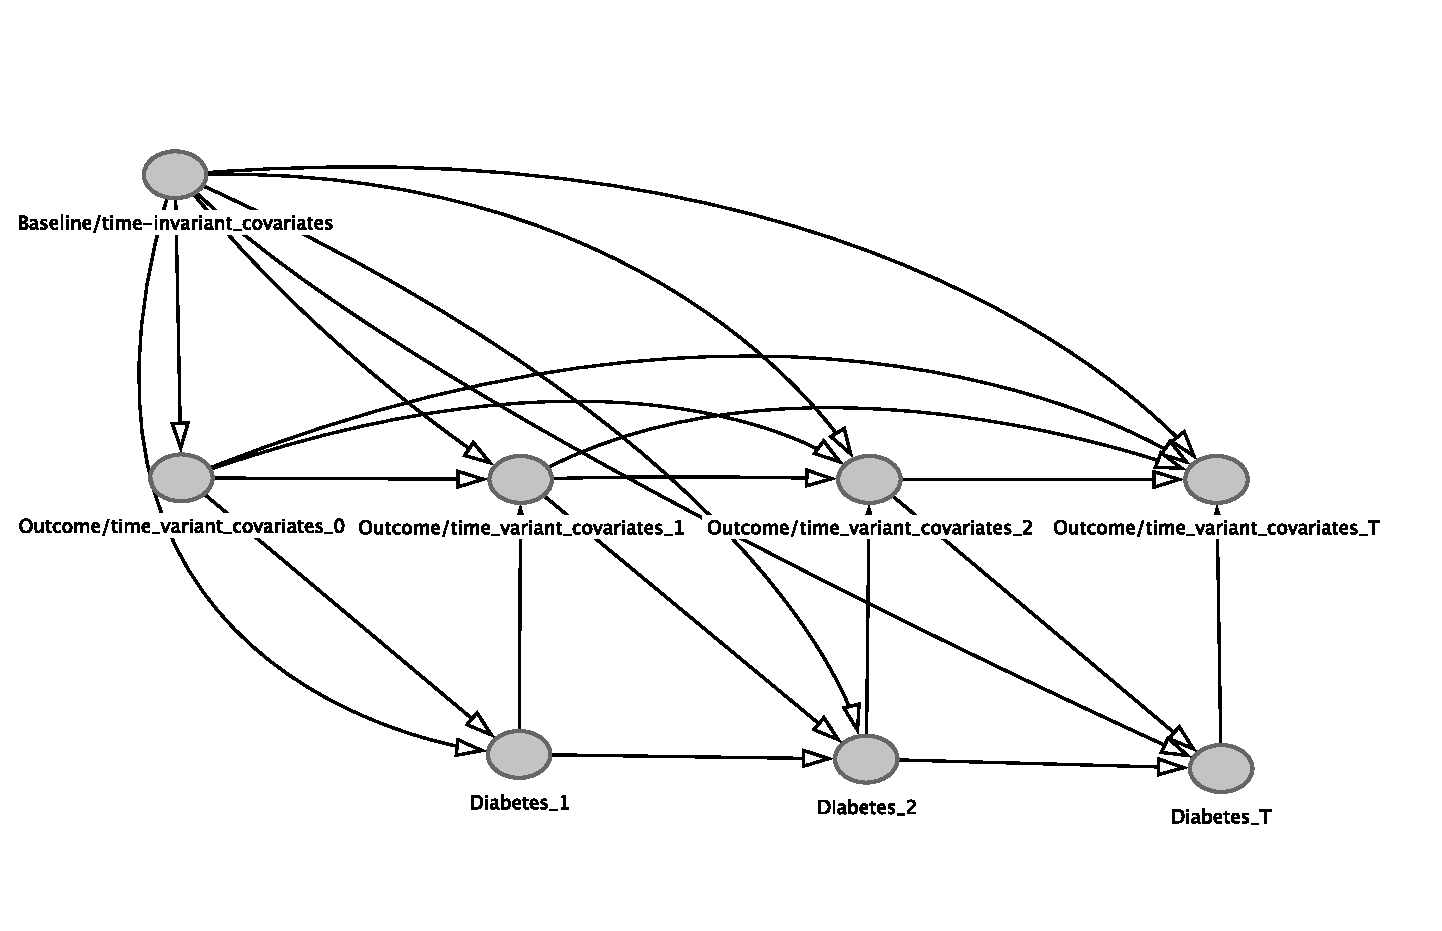
\includegraphics[width=\linewidth]{Chapter5/DAG/dag_msm_alt}
\end{center}
\footnotesize{\textit{Notes} \acp{MSM} assume the absence of unobserved time-invariant and unobserved time-variant confounders but allow the past treatments to affect the current outcomes  (arrows going from Diabetes to time-variant covariates in the same wave) and the past outcomes to affect the current treatment (arrows going from time-variant covariates to Diabetes).  Lagged time-variant covariates, baseline and time-invariant covariates predict current diabetes status.}
\end{figure}


Because \textit{unstabilized} \acp{IPTW} can be highly variable and therefore less precise, it is recommended to stabilize the weights, especially when the predicted probabilities of exposure are close to zero \parencite{Cole2008}. To calculate \textit{stabilized} \acp{IPTW}, \acp{IPTW} are created by predicting the diagnosis of diabetes using only baseline values of time-variant and time-invariant confounders as right-hand side variables. Similar to the calculation of \textit{unstabilized} \acp{IPTW}, cumulative probabilities are calculated by multiplying the predicted probabilities in the current and all previous waves, for each wave after the baseline wave. To calculate \textit{stabilized} \acp{IPTW} the just created weights are divided by the \textit{unstabilized} \acp{IPTW}. The resulting \textit{stabilized} \acp{IPTW} now only reflect the confounding due to the time-varying covariates, which cannot be appropriately adjusted for by standard regression models \parencite{Cole2008}. Because our analysis is stratified by males and females, we create separate weights for each gender.

The \acp{MSM} for any of the outcome variables are then estimated adjusting for any baseline and time-invariant confounders used in the calculation of the \acp{IPTW}, except for the respective outcome of interest, and weighted by the \textit{stabilized} \acp{IPTW} to adjust for time-variant confounding. \ac{OLS} regression models were used for continuous outcomes (\ac{BMI}, waist circumference and calorie consumption) and a logistic model for the binary outcomes (employment status, smoking status and alcohol consumption). For the logistic model we calculate average marginal effects for greater comparability with the results of the \ac{FE} models. Robust standard errors to account for intra-class correlation of repeated outcome measurements in individuals are used throughout. In our primary analysis, we present the results of the \ac{MSM} with untruncated stabilized weights, as these provide theoretically unbiased estimates, albeit they may be less efficient than truncated weights if the \acp{IPTW} have a wide range considerably diverting from 1 \parencite{Cole2008}. Given that our \acp{IPTW} do not include very extreme values and have a mean weight of 1 (see Table \ref{tab:stabweights}), using untruncated weights likely leads to very little loss in efficiency in our case, supporting the decision to use untruncated weights in our primary analysis.

\subsubsection{Fixed effects}

While the \ac{MSM} can account for pre-treatment selection on observable and time-variant confounders, it assumes that there are no unobserved time-invariant confounders such as family background, cognitive abilities, and other personal characteristics. This is a strong assumption that might be violated in practice. The individual level \ac{FE} model can help remedy this problem as it is able to account for both observed time-variant and invariant variables as well as time-invariant unobserved variables as shown in the \ac{DAG} in Figure \ref{fig:DAG_fe}. It does so by demeaning all covariates at each time point with the overall individual mean across all observed time points. It then uses solely the within-person variation for identification, thereby accounting for any time-invariant observed or unobserved as well as observed time-variant effects. 


This comes at a price: due to the demeaning, time-invariant variables, such as Han ethnicity, are dropped from the model and their association with the outcomes cannot be estimated. Further, because the \ac{FE} model is not able to account for any effects of a diabetes diagnosis on other time-variant confounders, only a more limited set of confounders can be included compared to the \ac{MSM}. Otherwise the estimates of the effect of a diabetes diagnosis would likely be biased due to the inclusion of 'bad controls'. Bad controls are control variables that have been affected by the treatment itself---such as \ac{BMI} or smoking status after a diabetes diagnosis---and therefore likely capture part of the causal effect of diabetes on the outcome of interest, biasing the diabetes coefficient \parencite{Angrist2009a}. Also age is dropped from our \ac{FE} estimations because in \ac{FE} models two or more variables that change at the same rate between waves cannot be separately identified. In our case this applies for age and time-dummies, as both variables increase by one unit each additional year \parencite{Wooldridge2012}. Consequently, for the estimation of the effect of time since diagnosis, we have to rely on the presence of people without diabetes in the sample, for which diabetes duration does not increase at the same rate as time. Our \ac{FE} specifications thus only include controls for age squared, the level of urbanization, education, being married, having any medical insurance, living in a rural area, region and time dummies as well as per capita household income.  \ac{FE} models also make another assumption, which has received much less attention, namely that there is no dynamic causal relationship between treatment and outcomes, i.e. that past treatments have no direct effect on current outcomes, and that past outcomes have no direct effect on current treatment. If this assumption is violated, then results based on \ac{FE} are biased \parencite{Imai2016}. Accordingly, the choice between the use of a \ac{FE} model or a \ac{MSM} depends on the trade-off between unobserved time-invariant confounding and dynamic causal relationships between diabetes and our outcome variables.\footnote{Because it is not possible to retrieve average marginal effects from a logistic \ac{FE} model, we prefer to use a linear \ac{FE} model instead. It generally produces very similar estimates compared to non-linear models \parencite{Angrist2009a}.}


\begin{figure}[!p]
\begin{center}
\caption{\label{fig:DAG_fe} Direct acyclic graph for the fixed effects model}
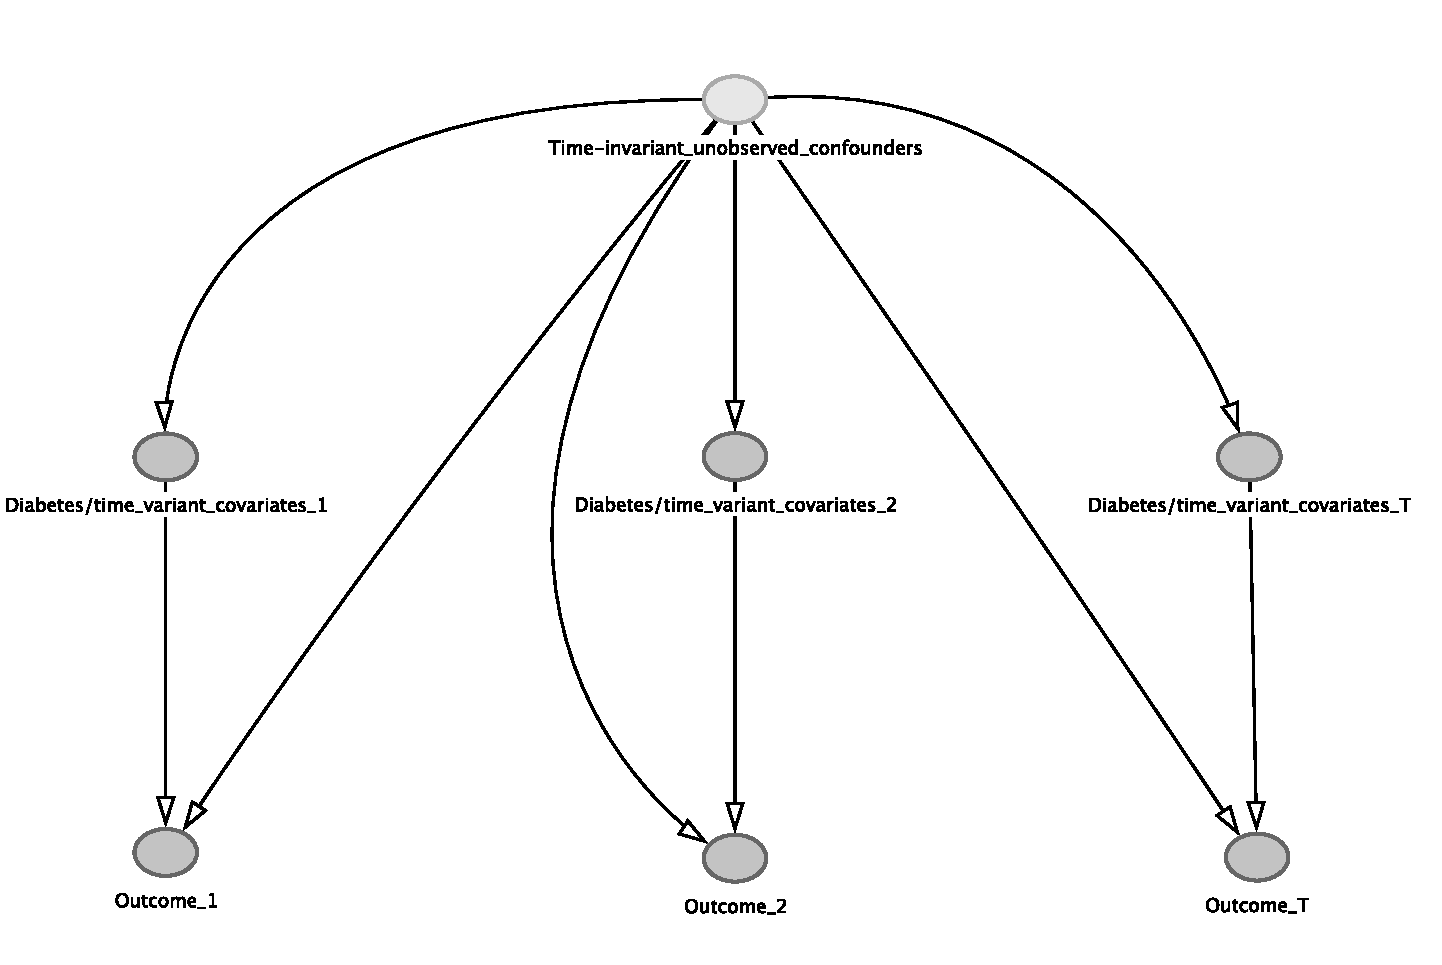
\includegraphics[width=\linewidth]{Chapter5/DAG/dag_fe_alt_corrections}
\end{center}
\footnotesize{\textit{Notes} \ac{FE} models account for time-invariant unobserved confounding (light grey circle), but still assume the absence of unobserved time-variant confounding. They further do not allow for past outcomes to affect the current treatment, i.e. diabetes status.}
\end{figure}


\subsubsection{Random effects}

Random effects assume, similar to the \ac{MSM}, no unmeasured confounding and, similar to the \ac{FE} model, no dynamic relationship between diabetes and our outcomes. Under these assumptions the \ac{RE} model is efficient and consistent, making it the preferable estimator if its assumptions are not violated. It is also preferable over the pooled \ac{OLS} estimator, as the \ac{RE} estimator takes into account the serial correlation of the errors across time \parencite{Wooldridge2012}. 

To discriminate between the \ac{RE} and \ac{FE} estimator, a robust Hausman test is carried out using the user written Stata command xtoverid. A rejection of the null hypothesis suggests that the underlying \ac{RE} assumptions are false and the \ac{FE} model should be used instead \parencite{Wooldridge2012}.\footnote{We use the original non-imputed data to carry out the Hausman test.} 



\subsubsection{Multiple imputation}

To avoid excluding participants with missing data on one or more variables, we used chained multiple imputation to impute the missing values in Stata 13 using the user written ICE command \parencite{Royston2009}. For most of the included variables, less than 10 percent of the observations was missing. Only the anthropometric measures of \ac{BMI} and waist circumference had both about thirteen percent missing data which had to be imputed (see Table \ref{tab:missing_data} in the appendix for detailed information on the number of missing observations). In total---before imputation---close to 20 percent of all cases were incomplete, i.e. had at least one variable that had missing data. Thirty imputed data sets were imputed, and the regression results obtained from each set were combined so as to ensure correct standard errors. In each imputed data set the imputed values of each missing variable varies randomly, centred on the value predicted for that record, so as to avoid spurious correlation between the variable and its predictors. When analysing multiply imputed data, increased precision is obtained by using more imputed data sets. Thirty imputed data sets is well above the commonly suggested rule of thumb that the number of imputations should be similar to the percentage of incomplete cases in the data (see for example \textcite{White2011,Bodner2008} for practical suggestions regarding the optimal number of imputations). Imputation models included all variables used in the \acp{MSM}. We imputed missing data in the same wave for which some data were recorded; we did not impute completely missing waves. Further, we assumed that once a diabetes diagnosis was reported, the individual had diabetes in every ensuing wave, even when the observation was missing. If diabetes was never reported in any wave, we assumed that the individual never had diabetes. We then only imputed missing values for those observations that had a non-missing diabetes status. For the calculation of the marginal effects in the \ac{MSM} logit models, Rubin's rules were applied using the user written Stata command mimrgns \parencite{Klein2014}.

\subsubsection{Numbers of observations}

Because we used lagged independent variables to construct the stabilized weights for the \acp{MSM}, the number of observations used in the \acp{MSM} is lower than those used in the \ac{FE} and \ac{RE} models, where we do not use lagged variables. The summary statistics shown in Table \ref{tab:descriptives_diab} are based on the observations used in the \ac{FE} models. The number of observations is stated below each table.

\subsubsection{Sensitivity analyses}

We conduct three additional sensitivity analyses in order to test the robustness of our results. First, we truncate weights at the 1\textsuperscript{st} and 99\textsuperscript{th} percentile to investigate the sensitivity of the \acp{MSM} to the most extreme weights. While untruncated weights provide unbiased estimates under the assumptions of the \ac{MSM}, they may not be the most efficient and tend to have larger standard errors \parencite{Cole2008}. Second, we estimate the \ac{FE} and \acp{MSM} using the original non-imputed data to ascertain the extent to which multiple imputation affected the results. Third, we report in the appendix the estimates of models using overweight and obesity instead of \ac{BMI} and waist circumference as the outcomes of interest, to investigate the effect of a diabetes diagnosis on changes in the probabilities to be overweight or obese.

\section{\label{sec:Results5}Results}

From the descriptive statistics (Table \ref{tab:descriptives_diab}), we can observe that people with diabetes in any wave are less likely to be employed. Looking at health behaviours, the prevalence of smoking and drinking is lower for men with diabetes; they also consume fewer calories compared to men without diabetes.  Note that it is mainly men who smoke and report alcohol consumption while very few women do so. Further, the diabetes group has both higher \ac{BMI} and waist circumference levels. They are also older, live in more urbanized areas, are more likely to have insurance and men are somewhat better educated while women are less educated compared to their counterparts without diabetes. Both men and women with diabetes report an average time since diagnosis of around 4.5 years. Looking at per capita household income, men and women with diabetes come from household with higher income levels than those without a diabetes diagnosis. Further, it appears that in China it is less educated women that report a diagnosis, while men with diabetes are better educated compared to those without diabetes.

Predicting the denominator for the stabilized weights (Table \ref{tab:predictors}) we find that for men a higher baseline \ac{BMI} increases the risk of a diabetes diagnosis. Further, increases in age, waist circumference as well as urbanization levels are associated with higher chances for men to be diagnosed with diabetes throughout the survey. Interestingly, becoming employed decreases the chances of being diagnosed with diabetes slightly, justifying the use of the \ac{MSM} in our employment models as well  . Because these are not causal estimates, it may be that it is more likely for men with a lower risk of diabetes to select into employment.
\begin{landscape}
\begin{table}[p]
\caption{\label{tab:descriptives_diab}Sample means for males and females, by diabetes status}
\begin{center}
\begin{adjustbox}{max width=\linewidth}  
{
\def\sym#1{\ifmmode^{#1}\else\(^{#1}\)\fi}
\begin{tabular}{l*{6}{SS}}
\toprule
                    &\multicolumn{3}{c}{Males}             &\multicolumn{3}{c}{Females}           \\\cmidrule(lr){2-4}\cmidrule(lr){5-7}
                    &\multicolumn{1}{c}{No diabetes}&\multicolumn{1}{c}{Diabetes}&\multicolumn{1}{c}{p-value (t-test)}&\multicolumn{1}{c}{No diabetes}&\multicolumn{1}{c}{Diabetes}&\multicolumn{1}{c}{p-value (t-test)}\\
\midrule
Employed            &        82\%&        68\%&    <0.001        &        67\%&        29\%&     <0.001       \\
Smokes              &        58\%&        47\%&      <0.001      &        3\%&        4\%&    0.409        \\
Any alcohol consumption&     63\%&        53\%&       <0.001     &        9\%&        4\%&   <0.001         \\
Daily Kcal eaten (3-day average)&     2422&     2166&      <0.001      &     2068&     1931&   0.001         \\
BMI                 &       22.99&      24.90&       <0.001     &       23.10&       25.80&    <0.001        \\
Waist circ. (cm)    &       82.02&       88.81&      <0.001      &       78.80&       87.55&     <0.001       \\
Age                 &       42.27&      52.76&      <0.001      &       43.24&       55.32&     <0.001       \\
Han ethnicity       &        87\%&      89\%&     0.292       &        87\%&        93\%&     0.002      \\
Rural area          &        69\%&       52\%&     <0.001       &        68\%&        51\%&     <0.001       \\
Married             &        83\%&      93\%&     <0.001       &        88\%&        87\%&    0.392        \\
Secondary education     &        65\%&      68\%&   0.439         &        50\%&        43\%&       0.007     \\
University education    &        5\%&      11\%&    <0.001        &        4\%&        1\%&     0.017      \\
Any health insurance&        51\%&     82\%&     <0.001       &        50\%&        71\%&       <0.001      \\
Urbanization Index  &       60.87&     74.48&     <0.001       &       61.77&       68.68&     <0.001       \\
Per capita household income (Yuan (2011))&    8617&     16328&    <0.001        &     8581&     11101&    <0.001        \\
Years since diabetes diagnosis&       -&        4.5&      -      &        -&        4.65&      -      \\
\midrule
Observations        &       23159&         284&       &        23369&         333&            \\
\bottomrule
\end{tabular}
}
\end{adjustbox}
\end{center}
\end{table}
\end{landscape}
Higher household income levels are not predictive of a diagnosis for men or women, despite what the descriptive statistics indicated. For women, higher age and waist circumference at baseline, increases in \ac{BMI} as well as living in a non-rural environment predict a diabetes diagnosis. 

\begin{table}[p]
\caption{\label{tab:predictors}Time variant and invariant predictors of a diabetes diagnosis  (denominator of stabilized weights): logistic regression models}
\begin{center}
\begin{adjustbox}{max width=\linewidth} 
\begin{threeparttable}  %adds notes to tables 
{
\def\sym#1{\ifmmode^{#1}\else\(^{#1}\)\fi}
\begin{tabular}{l*{4}{S S}}
\toprule
                &\multicolumn{2}{c}{Males}&\multicolumn{2}{c}{Females}\\\cmidrule(lr){2-3}\cmidrule(lr){4-5}&\multicolumn{1}{c}{(1)}&\multicolumn{1}{c}{(2)}&\multicolumn{1}{c}{(3)}&\multicolumn{1}{c}{(4)}\\
                &\multicolumn{1}{c}{$\beta$}&\multicolumn{1}{c}{SE}&\multicolumn{1}{c}{$\beta$}&\multicolumn{1}{c}{SE}\\
\midrule
Age (bl)          &-.000 &.001         &.004\sym{**} & .002         \\
Age squared (bl)       &.000 &.000         &-.000\sym{**} &.000         \\
\ac{BMI} (bl)        &.001\sym{***} &.000         &.001 &.000         \\
Waist circumference (cm) (bl)        &.000 &.000         &.000\sym{*} &.000         \\
3-Day Ave: Energy (kcal) (bl)       &-.000 &.000         &.000 &.000         \\
Smoking (bl)    &.001 &.002         &.003 &.006         \\
Alcohol consumption (bl)        &.003\sym{*} &.002         &.000 &.005         \\
Urbanization index (bl)      &-.000 &.000         &-.000 & .000         \\
Secondary educ. (bl)    &-.001 &.003         &.003 &.003         \\
University educ. (bl) &-.000 &.006         & - & -         \\
Married (bl)      &-.002 &.004         &-.000 &.004         \\
Any medical insurance (bl)    &.002 &.002         &-.000 &.002         \\
Employed (bl)        &.002 &.003         &.001 &.002         \\
Han ethnicity   &.001 &.003         &-.002 &.003         \\
Rural      &-.001 &.002         &-.005\sym{***} &.002         \\
Per capita household income (2011 Yuan) (bl)&-.000 &.000         &-.000 &.000         \\
Survey year && \\
\hspace*{10mm}2004&.002 &.002         &-.001 &.002         \\
\hspace*{10mm}2006&.003 &.002         &-.003 &.003         \\
\hspace*{10mm}2009&.009\sym{***} &.003         &-.001 &.004         \\
\hspace*{10mm}2011&.001 &.003         &.001 &.004         \\
Age           &.003\sym{**} &.001         &-.002 &.002         \\
Age squared        &-.000\sym{**} &.001         &.000 &.000         \\
BMI          &-.001 &.000        &.001\sym{**} &.000         \\
Waist circumference (cm)         &.000 &.000         &-.000 &.000         \\
3-Day Ave: Energy (kcal)        &-.000 &.000         &-.000 &.000         \\
Smoking         &-.003 &.002         &.000 &.006         \\
Alcohol consumption        &-.004\sym{**} &.002         &-.003 &.006         \\
Urbanization index         &.000 &.000         &.000 &.000         \\
Secondary education     &.001 &.003         &.000 &.003         \\
University education    &.001 &.006         & - & -         \\
Married       &-.000 &.004         &-.003 &.004         \\
Any medical insurance     &.001 &.002         &-.001 &.002         \\
Employed         &-.004\sym{**} &.002         &-.003 &.002         \\
Per capita household income (2011 Yuan) (2011 Yuan) &.000 &.000         &-.000 &.000         \\
\bottomrule
\end{tabular}
\begin{tablenotes}
\item \footnotesize \textit{Notes} Average marginal effects based on logistic regression. Results for province dummies omitted to preserve space. University education was dropped in the female sample as having university education perfectly predicted diabetes status. N=16047 (male sample), N=16658 (female sample). \sym{*} \(p<0.10\), \sym{**} \(p<0.05\), \sym{***} \(p<0.01\). \\
\end{tablenotes}
}
\end{threeparttable}

\end{adjustbox}
\end{center}
\end{table}



\begin{table}[p]
\caption{\label{tab:binary}Analysis of the effect of a diabetes diagnosis on employment status and behavioural outcomes using MSM, FE and RE}
\begin{adjustbox}{max width=\linewidth, center}
\begin{threeparttable}  %adds notes to tables
{
\def\sym#1{\ifmmode^{#1}\else\(^{#1}\)\fi}
\begin{tabular}{l*{6}{S
S}}
\toprule
                &\multicolumn{1}{c}{(1)}&\multicolumn{1}{c}{(2)}&\multicolumn{1}{c}{(3)}&\multicolumn{1}{c}{(4)}&\multicolumn{1}{c}{(5)}&\multicolumn{1}{c}{(6)}\\
                &\multicolumn{1}{c}{Employment}&\multicolumn{1}{c}{Smoking}&\multicolumn{1}{c}{Alcohol}&\multicolumn{1}{c}{BMI}&\multicolumn{1}{c}{Waist (cm)}&\multicolumn{1}{c}{Calories (kcal)}\\
                \midrule
&\multicolumn{6}{c}{\emph{Marginal structural model}} \\  
\addlinespace                                   

Male sample &&&&&&\\
Diabetes&      -.009         &    -.070\sym{**} &    -.094\sym{***}&    -.735\sym{***}&   -1.887\sym{***}& -135.061\sym{**} \\
                &   (.026)         &   (.032)         &   (.036)         &   (.180)         &   (.574)         & (58.593)         \\
Female sample &&&&&&\\
Diabetes     &     -.117\sym{***}&    -.015\sym{*}  &    -.029\sym{**} &    -.388         &    -.335         &  -45.630         \\
                &   (.029)         &   (.008)         &   (.012)         &   (.240)         &   (.631)         & (33.530)         \\    
\midrule      
\addlinespace 
&\multicolumn{6}{c}{\emph{Fixed effects}} \\
\addlinespace             
Male sample &&&&&&\\
Diabetes        &      .022         &    -.023         &    -.104\sym{***}&    -.715\sym{***}&   -2.217\sym{***}& -168.297\sym{***}\\
                &   (.030)         &   (.032)         &   (.036)         &   (.183)         &   (.610)         & (62.115)         \\
Female sample &&&&&&\\
Diabetes        &    -.112\sym{***}&    -.027\sym{**} &    -.012         &    -.644\sym{**} &   -1.251\sym{**} &  -61.175         \\
                &   (.035)         &   (.013)         &   (.010)         &   (.263)         &   (.616)         & (47.420)         \\ 
\midrule      
\addlinespace                 
&\multicolumn{6}{c}{\emph{Random effects}} \\
\addlinespace             
Male sample &&&&&&\\
Diabetes        &    -.022         &    -.064\sym{**} &    -.104\sym{***}&    -.379\sym{**} &    -.756         & -172.467\sym{***}\\
                &   (.028)         &   (.029)         &   (.029)         &   (.177)         &   (.542)         & (48.768)         \\
Female sample &&&&&&\\
Diabetes        &    -.152\sym{***}&    -.021\sym{**} &    -.019\sym{***}&    -.263         &     .459         &  -39.267         \\
                &   (.027)         &   (.011)         &   (.006)         &   (.247)         &   (.570)         & (34.256)         \\                            
\bottomrule
\end{tabular}
\begin{tablenotes}
\item \footnotesize \textit{Notes} The coefficients of the MSM for outcomes 1--3 represent average marginal effects based on logistic regression models. All other coefficients are from linear regression models. Robust standard errors in parentheses. Other control variables for FE/RE: Age squared, region, urban, education, Han ethnicity, marital status, urbanization index, time dummies, health insurance status, household expenditures. RE additionally controls for age. MSM controls for baseline values of the same variables as the FE/RE models additionally to baseline values of age, alcohol consumption, smoking status, BMI, waist circumference and calorie consumption.  Fixed/random effects: N=23443 (male sample), N=23702 (female sample); MSM:  N=16047 (male sample), N=16658 (female sample). \sym{*} \(p<0.10\), \sym{**} \(p<0.05\), \sym{***} \(p<0.01\).
\end{tablenotes}
}
\end{threeparttable}
\end{adjustbox}

\end{table}
The results of our regression analysis are presented in Table \ref{tab:binary}. Both the \acp{MSM} and \ac{FE} models indicate that women with a diabetes diagnosis have lower probabilities of being employed than their counterparts without diabetes, with a reduction of 11.7 percentage points in the \ac{MSM} and 11.2 percentage points in the \ac{FE} model. This translates into a relative reduction in employment probabilities between 16--17\%. For men no such effect is observed.



A more ambiguous picture is painted for the effect of a diabetes diagnosis on behavioural risk factor outcomes. According to the \ac{MSM}, for males a diabetes diagnosis leads to smoking cessation, reductions in alcohol consumption as well as \ac{BMI}, waist circumference and calorie consumption. Results for women look different. While the point estimates indicate a reduction in all outcomes, these tend to be smaller than those for men and only exhibit strong statistical significance for smoking cessation and alcohol consumptions, factors where women already have a very low prevalence. Compared to the \ac{MSM}, the \ac{FE} model finds similar effects for men, apart from a less important effect on smoking cessation.	For women, however, it finds much larger, and statistically significant, reductions in \ac{BMI} and waist circumference compared to the \ac{MSM}. 

The results of the \ac{RE} models shows an even stronger effect of diabetes on female employment probabilities and  smaller reductions in male and female \ac{BMI} and waist circumference, even suggesting a positive association between a diabetes diagnosis and female waist circumference. For the other outcomes, results are very similar to those from the \acp{MSM} and \ac{FE} models. Nonetheless, the Hausman test still rejects the use of the \ac{RE} model throughout (see Table \ref{tab:binary_non_mi}).

Exploring the effect of a diabetes diagnosis over time, we first estimate a specification using time since diagnosis as a continuous variable. The results of the \acp{MSM} (Table \ref{tab:duration}) indicate a steady reduction of female employment probabilities of close to two percentage points per year and of male alcohol consumption, \ac{BMI}, waist circumference and calorie consumption. The \ac{FE} model again supports the finding of the \ac{MSM}, showing very similar, though somewhat larger effects in terms of size and statistical significance. The evidence for changes in risk factors for females is less consistent across models and outcomes, with the \ac{MSM} suggesting almost no effects while the \ac{FE} model indicates a reduction in \ac{BMI}. The effect sizes for changes in health behaviours in women are consistently lower than those found for men. 

The \ac{RE} models again find larger effects on female employment probabilities and a smaller impact of a diabetes diagnosis on reductions in \ac{BMI} and waist circumference for both sexes. 


\begin{table}[p]
\caption{\label{tab:duration}Analysis of the effect of each year since diabetes diagnosis on employment status and behavioural outcomes using MSM, FE and RE}
\begin{adjustbox}{max width=\linewidth} 
\begin{threeparttable}  %adds notes to tables
{
\def\sym#1{\ifmmode^{#1}\else\(^{#1}\)\fi}
\begin{tabular}{l*{6}{S S}} \toprule
                &\multicolumn{1}{c}{Employment}&\multicolumn{1}{c}{Smoking}&\multicolumn{1}{c}{Any alcohol}&\multicolumn{1}{c}{\ac{BMI}}&\multicolumn{1}{c}{Waist (cm)}&\multicolumn{1}{c}{Calories (kcal)}\\
                \midrule
&\multicolumn{6}{c}{\emph{Marginal structural model}} \\
\addlinespace                     
Male sample &&&&&&\\
Time since diagnosis&    -.003         &    -.010\sym{*}  &    -.014\sym{**} &    -.127\sym{***}&    -.340\sym{***}&  -21.770\sym{**} \\
                &   (.004)         &   (.005)         &   (.007)         &   (.031)         &   (.099)         &  (9.842)         \\
Female sample &&&&&&\\
Time since diagnosis&      -.017\sym{***}&    -.002         &    -.004         &    -.066\sym{*}  &    -.072         &   -8.735         \\
                &   (.005)         &   (.001)         &   (.003)         &   (.040)         &   (.109)         &  (5.589)         \\
\addlinespace 
\midrule
&\multicolumn{6}{c}{\emph{Fixed effects}} \\               
\addlinespace
Male sample &&&&&&\\
Time since diagnosis   &  -.001         &    -.003         &    -.017\sym{**} &    -.150\sym{***}&    -.520\sym{***}&  -22.286\sym{**} \\
                &   (.007)         &   (.006)         &   (.007)         &   (.037)         &   (.121)         & (11.083)         \\
Female sample &&&&&&\\
Time since diagnosis  & -.019\sym{***}&    -.003         &    -.000         &    -.102\sym{***}&    -.215\sym{*}  &   -6.747         \\
                &   (.007)         &   (.002)         &   (.001)         &   (.039)         &   (.117)         &  (7.028)         \\                 
\midrule      
\addlinespace                 
&\multicolumn{6}{c}{\emph{Random effects}} \\
\addlinespace             
Male sample &&&&&&\\
Diabetes        &    -.006         &    -.009\sym{*}  &    -.015\sym{***}&    -.099\sym{***}&    -.269\sym{***}&  -24.703\sym{***}\\
                &   (.006)         &   (.006)         &   (.005)         &   (.035)         &   (.096)         &  (8.655)         \\
Female sample &&&&&&\\
Diabetes        &     -.023\sym{***}&    -.002         &    -.002\sym{**} &    -.056         &     .013         &   -6.444         \\
                &   (.006)         &   (.002)         &   (.001)         &   (.039)         &   (.114)         &  (5.670)         \\ 
\bottomrule
\end{tabular}
\begin{tablenotes}
\item \footnotesize \textit{Notes} The coefficients of the MSM for outcomes 1--3 represent average marginal effects based on logistic regression models. All other coefficients are from linear regression models. Other control variables for FE/RE: Age squared, region, urban, education, Han ethnicity, marital status, urbanization index, time dummies, health insurance status, household expenditures. RE additionally controls for age. MSM controls for baseline values of the same variables as the FE/RE models additionally to baseline values of age, alcohol consumption, smoking status, BMI, waist circumference and calorie consumption. FE/RE: N=23443 (male sample), N=23702 (female sample); MSM:  N=16047 (male sample), N=16658 (female sample). \sym{*} \(p<0.10\), \sym{**} \(p<0.05\), \sym{***} \(p<0.01\).
\end{tablenotes}
}
\end{threeparttable}
\end{adjustbox}
\end{table}


In a second step we estimate a specification using year dummies to capture the potential non-linearity in the relationship between time since diagnosis and our outcomes. The results for the different estimation methods are visualized in Figures \ref{fig:duration_g_msm_mi} and \ref{fig:duration_g_fe_mi} and presented in Tables \ref{tab:duration_groups_msm}, \ref{tab:duration_groups_fe} and \ref{tab:duration_groups_re} in the appendix for the \ac{MSM}, \ac{FE} and \ac{RE} model, respectively.  The \ac{MSM} and \ac{FE} model indicate a statistically significant reduction in female employment probabilities in the first eight years after diagnosis, with the exception of the fifth and sixth year, where the effects are not statistically significant. Further, male \ac{BMI} and waist circumference are also reduced significantly in most years especially in the \ac{FE} models which finds significant effects in the first six years after diagnosis and then in years nine to twelve. The \ac{MSM} still indicates reductions but these tend to be less statically significant. Calorie consumption is not found to be statistically significantly reduced in a consistent manner either in the \ac{MSM} or the \ac{FE} model. Behavioural risk factors for women are again not found to be reduced consistently, apart from \ac{BMI} where some trend towards a reduction over time is visible. Interestingly, female employment already decreases rapidly in the first to second year after diagnosis and it does not appear that females are able to increase their employment probabilities later on. Unfortunately it was not possible to estimate the effects on female smoking and alcohol consumption due to the low prevalence of these risk factors in females and the lower sample size in the \ac{MSM}. Using the \ac{FE} model, all point estimates indicate similar effects. The \ac{RE} model, again suggests larger effects on female employment and lower effects on \ac{BMI} and waist circumference than both other estimation methods. 

The sensitivity analyses using truncated weights shows very similar effects to those using the untruncated weights (Tables \ref{tab:truncation} and \ref{tab:duration_groups_tr} in the appendix), suggesting no important bias and supporting the decision to use untruncated weights. The results using non-imputed data are broadly similar (Tables \ref{tab:binary_non_mi}, \ref{tab:duration_non_mi}, \ref{tab:duration_groups_non_mi_msm}, \ref{tab:duration_groups_non_mi_fe} and \ref{tab:duration_groups_non_mi_re} in the appendix), in particular for the \ac{FE} model, and also indicate a reduction in female employment probabilities and male alcohol consumption, \ac{BMI} and waist circumference. The coefficients of the \ac{MSM} still point into the same direction as those using the imputed data, but the estimated effects are smaller in size and confidence intervals are relatively large. The \ac{RE} model still shows a stronger effect on female employment probabilities and smaller reductions in especially the weight measures \ac{BMI} and waist circumference. Using overweight and obesity instead of \ac{BMI} and waist circumference as indicators for weight changes, we do not find as consistent reductions in weight status for men as we did using the continuous estimates (Tables \ref{tab:obesity_binary} and \ref{tab:obesity_dur} and Figure \ref{fig:obesity_duration_g} in the appendix). Nonetheless, the point estimates still show a reduction in obesity, in particular over time and for men, supporting the reductions found using continuous measurements.\footnote{The coefficients for overweight are difficult to interpret as it is unclear if the negative coefficient is caused by people transferring into obesity or into normal weight.}

\begin{landscape}
\begin{figure}
\begin{center}
\caption{\label{fig:duration_g_msm_mi} The effect of time since diabetes diagnosis on employment, smoking and alcohol consumption (duration groups)}
\makebox[\linewidth]{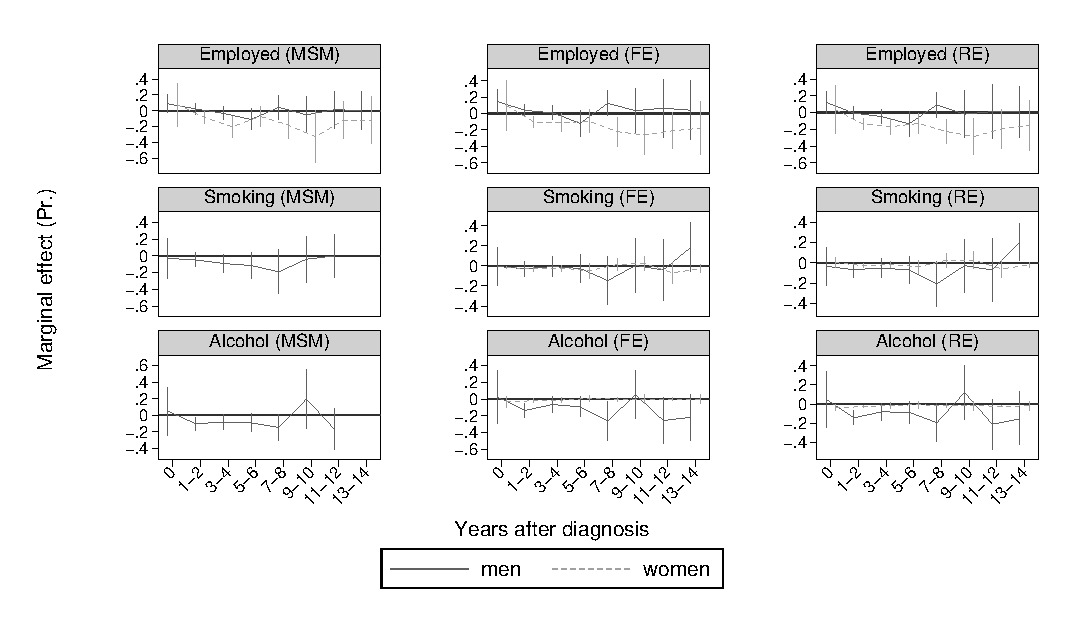
\includegraphics[width=\linewidth,height=\textheight]{Chapter5/Figures/binary.eps}}
\end{center}
\footnotesize\textit{Note} The visualized coefficients are based on the results of the regression models shown in Tables \ref{tab:duration_groups_msm} and \ref{tab:duration_groups_fe} in the appendix. 95\% confidence intervals.

\end{figure}
\begin{figure}
\begin{center}
\caption{\label{fig:duration_g_fe_mi} The effect of time since diabetes diagnosis on BMI, waist circumference and calorie consumption (duration groups)}
\makebox[\linewidth]{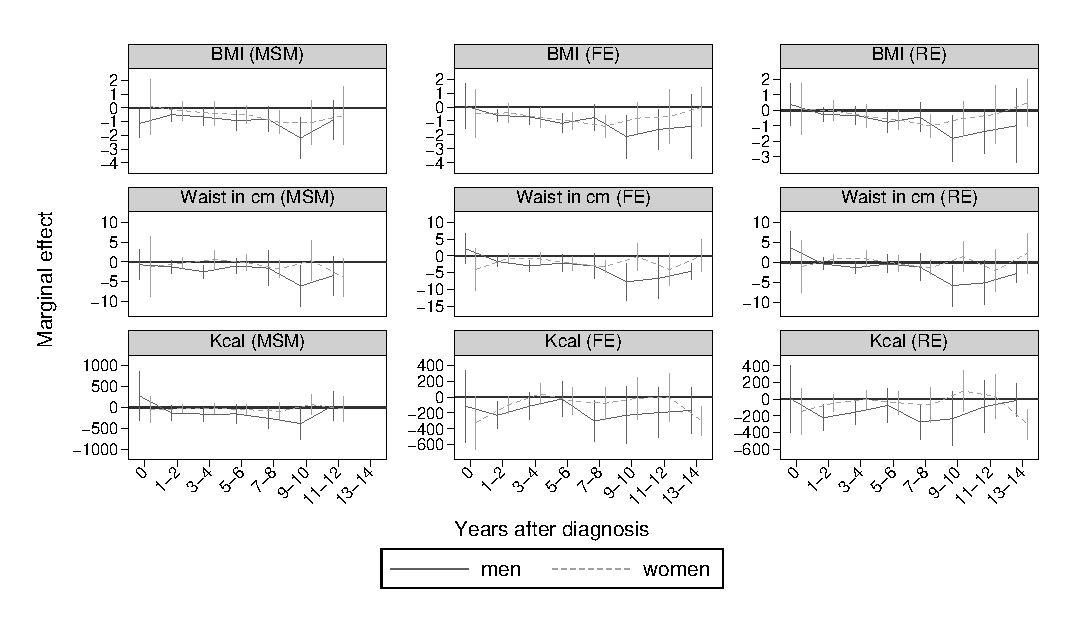
\includegraphics[width=\linewidth,height=\textheight]{Chapter5/Figures/continuous.eps}}
\end{center}
\footnotesize\textit{Note} The visualized coefficients are based on the results of the regression models shown in Tables \ref{tab:duration_groups_msm} and \ref{tab:duration_groups_fe} in the appendix. 95\% confidence intervals.

\end{figure}
\end{landscape}


\section{\label{sec:Discussion5}Discussion}

The evidence for the impact of a diabetes diagnosis on employment probabilities and behavioural risk factors remains scarce, in particular in \acp{MIC}, where diabetes has become a mayor contributor to the burden of disease. We added to this evidence by exploring these relationships using longitudinal data from China, also improving upon previously used methodologies by taking into account the potential relationship over time between diabetes and these outcomes.

Our results suggest that receiving a diabetes diagnosis in China leads to a strong and lasting reduction in female, but not male, employment probabilities. We also found reductions in male \ac{BMI} and waist circumference, alcohol and calorie consumption and potentially smoking to be associated with a diabetes diagnosis. We did not, however, find similar changes in behavioural risk factors for women. Accordingly, it appears that women in China have to endure stronger adverse labour market effects of diabetes and at the same time are less successful then men at making risk behaviour changes to reduce their risk of diabetes complications.

The \acp{MSM} and \ac{FE} models indicated very similar results suggesting that they are robust and that time-invariant confounding factors may play a limited role over and above baseline and time varying confounding factors. The \ac{MSM} results suggest that in particular \ac{BMI} and waist circumference levels as well as employment status can cause selection into a diabetes diagnosis and are then later themselves affected by the diagnosis, justifying the use of a \ac{MSM}. The \ac{RE} models further indicated that insufficiently accounting for confounding can---at least in this setting---lead to an overestimation of the impact of diabetes on employment status and an underestimation of the effects of a diagnosis on weight measures (\ac{BMI} and waist circumference). However, confounding may only be of limited relevance for  alcohol consumption, where the \ac{RE} models showed very similar results.

\subsection{Limitations}

The study has several limitations. While we used two estimation methods to reduce the influence of observed and unobserved confounding, respectively, none of the models is able to account for both forms of confounding. Therefore a causal interpretation is only possible under restrictive assumptions, namely no unobserved time-variant confounding for the \ac{FE} model and positivity, exchangeability and consistency for the \ac{MSM}. The assumption of positivity is likely to hold, given that every person should have at least a small chance of receiving a diabetes diagnosis. This is also supported by the relatively small range of stabilized weights and absence of zero-weights. The assumption of exchangeability or no unmeasured confounding could potentially be violated if not all time-invariant and time-variant confounders were accounted for, but this cannot be known for certain from existing data. We tested for part of this assumption by estimating a \ac{FE} model and, given that the results remained very similar, this suggests that unobserved time-invariant confounding may be of limited relevance in this case, even though this remains speculative as the Hausman test indicated some time-invariant confounding. Consistency would have been violated if a diabetes diagnosis had been reported but the person had actually not been diagnosed with diabetes. This was likely only violated in very rare cases of misreporting, given that specificity of diabetes self-report is very high in China \autocite{Yuan2015}. Because we were interested in the effect of a diabetes diagnosis, unobserved diabetes did not violate the consistency assumption.

A limitation of the \ac{FE} model is the possibility of time-variant confounding due to prior outcomes (for example employment status) affecting the current treatment (a diabetes diagnosis). We found some evidence that prior outcomes could affect selection into a diabetes diagnosis, potentially introducing bias in our \ac{FE} estimates. Given that the \ac{FE} estimates were close to those of the \acp{MSM}, it could be that this bias may not have been very strong. Overall, it remains difficult to pin down the potential source of a potential bias as, for example in the female employment models, both the \ac{MSM} and the \ac{FE} results are very similar while the \ac{RE} results indicate a somewhat bigger adverse effect. We have some evidence for both models that their underlying assumptions may not hold, with the Hausman test suggesting time-invariant confounding and the results of Table \ref{tab:predictors} indicating some time-variant confounding due to prior outcomes.

Finally, a limitation is that in this study we only observe the combined effect of all that entails a diabetes diagnosis.  However, a diabetes diagnosis can entail a variety of 'treatments' that are difficult to disentangle and may each have a distinct effect on the explored outcomes. 

\subsection{Potential mechanisms}

The effects of diabetes on employment and behaviour could work through several mechanisms. Firstly, the provision of information at diagnosis, may causes increases in stress and anxiety, but could also reduce anxiety by providing an explanation for the experienced symptoms \parencite{Peel2004}, with both potentially affecting productivity. Secondly, a diagnosis is also the starting point for medical treatment, which could help to alleviate symptoms and to lose weight, but also poses new challenges, in particular if treatment entails the exogenous provision of insulin or adherence to strict meal plans, likely adding to the burden of diabetes in daily life \parencite{vijan2005,Pibernik-Okanovic1996}. Thirdly, adherence to medical treatment may be heterogeneous across people with diabetes, with non-adherence likely leading to a further worsening of risk factors for complications, while good adherence may prevent or delay debilitating complications \parencite{Asche2011}. Fourthly, a diagnosis may also cause lifestyle changes such as increasing exercise levels, eating healthier and reducing smoking or alcohol consumption, all potentially affecting the risk of developing further complications and of changes in productivity. In the current study, it is not possible to ascertain the role of each of these factors in affecting employment probabilities and behavioural risk factors. Only for the reductions in smoking and alcohol consumption, it seems reasonable to attribute them to diagnosis induced awareness of the need to reduce these risk factors, as other pathways appear less likely to be relevant. 

The found adverse effect of diabetes on employment is in line with other studies on the labour market impact of diabetes that have found diabetes to reduce employment probabilities for women \parencite{Minor2011,Latif2009,Harris2009,Seuring2016}---often more than for men. Most comparable to our results are likely the results from Mexico in Chapter \ref{cha:Mex2}, which were also based on \ac{FE} estimations and data for a similar time period \parencite{Seuring2016}. The study found significant reductions for both males and females of about 5 percentage points. Taking into account the lower overall employment rate of Mexican women compared to men, this translated into a 16\% reduction in female employment probabilities, a figure comparable to the effect on Chinese women. However, in Mexico also men experienced adverse effects, unlike to what we found for China.

The found effects on changes in behavioural risk factors can be compared to the study by \textcite{Slade2012}. Slade finds reductions in alcohol consumption and smoking, though it appears that these reductions were not maintained over a longer time period. Unfortunately, Slade only provided information for the entire sample and the male sample, so that we cannot compare them directly with our results for women. In terms of the effect on weight, again both studies cannot be directly compared because Slade investigated the effect of a diagnosis on being overweight or obese, while we used continuous weight measures in our primary analysis due to the discussed difficulties of defining cut-off values for Asian populations. Slade found an initial reduction in weight status, but also that people with diabetes tended to become more likely to be overweight or obese after some time. Our results using overweight and obesity could tentatively be interpreted to indicate a more constant reduction in obesity over time, suggesting that reductions in weight in Chinese men may be longer lived than in the USA. Importantly---and in concordance with our findings---he found that simple covariate adjustment led to biased estimates of the impact on weight status, finding a positive relationship. This underlines the importance of accounting for potential sources of confounding.

The permanent reduction in male \ac{BMI} and waist circumference we have found has also been observed in a cohort of Danish patients \autocite{DeFineOlivarius2015}, where weight increased in the years preceding diagnosis, while after diagnosis weight decreased. The exact reasons for this decrease were unknown but attributed to motivation changes as a result of the diagnosis, concluding that the time around the diagnosis may represent a window of opportunity to obtain long lasting weight change. Nonetheless, reductions in weight may also be the result of treatment initiation with metformin or other diabetes drugs that have been shown to lead to weight reductions \autocite{Yang2014}. Importantly, the reduction in male \ac{BMI} levels and waist circumference were accompanied by reduced energy intake, suggesting that the changes in weight were at least partly the result of lower energy intake.  Further, given that in China diabetes incidence has been especially attributed to a high accumulation of visceral fat and central obesity \autocite{Ma2014}, the reductions in waist circumference may have had a particular positive effect on diabetes control and the prevention of comorbidities. Together, the lower levels of energy intake and waist circumference after the diagnosis allow for the interpretation that the reductions in \ac{BMI} were due to fat loss and not lower lean body mass \autocite{Klein2007}. 

For women, however, we did not find similar strong evidence for reductions in \ac{BMI}, waist circumference or energy intake. The relatively smaller effects for women could indicate a lower ability to change behaviours supportive of weight loss. This appears to be supported by the smaller reductions in energy intake. This could have---at least partly---contributed to a higher risk for diabetes complications further down the line, also adversely affecting employment probabilities. Apart from this, other explanations for the lower weight loss and larger employment penalty for women compared to men include their lower educational attainment, which has been indicated as a factor in preventing better glucose control \autocite{Luo2015} and may also affect the ability to successfully change behaviours. Lower income levels for females compared to men may also have negatively affected the ability to receive adequate treatment following a diagnosis, limiting their ability to change health behaviours \autocite{Luo2015}, increasing the risk of complications. We found that women with diabetes lived in households with lower income levels compared to men with diabetes, however, these income levels were still higher then for those without diabetes. Nonetheless, it may still be the case that women were less likely to access care due these differences in income. Moreover, there are likely biological factors that lead to worse health outcomes for women compared to men. There is some evidence that, due to different ways of fat storage between men and women, men tend to cross the diabetes threshold at an earlier point in time and at a comparatively healthier metabolic state then women \parencite{Peters2015,Peters2014a,Peters2014}. Women are more likely to have spend more time in a pre-diabetes state \parencite{Bertram2010} and to cross the threshold only once their metabolic health has significantly deteriorated, leading to a greater risk of cardiovascular disease and stroke \parencite{Peters2015}. Supporting this, a study for China found a greater prevalence of diabetes comorbidities in Chinese women compared to men \autocite{Liu2010}. In this light it may not be surprising that we find more conclusive evidence of worsening employment probabilities for women. If women are less likely to receive proper treatment and to change their health behaviours and at the same time have a greater risk for complications then men, the long term effects of diabetes on their health are likely more severe than for men and consequently affect their employment status to a greater extent.

Taken together, these estimation results suggest a lower risk of unemployment for men with diabetes potentially due to their greater ability to reduce behavioural risk factors, while the effect of diabetes on employment for women is substantial because no such changes in behaviour take place. Further analysis is needed to test this formally, and is beyond the scope of this paper.





\section{Conclusion}

Our results indicate worse outcomes for women then men after a diabetes diagnosis, with women experiencing a reduction in employment probabilities accompanied by and potentially partly due to an inability to reduce important risk factors for diabetes complications. For males, the opposite pattern is found, as they do not experience adverse employment effects and are able to achieve reductions in the investigated risk factors. These findings are robust to the application of two distinct, but complementary econometric techniques. Overall, given the large prevalence of undiagnosed diabetes, our results indicate that an early diagnosis may be a good way to foster early behaviour change that could lead to more positive health and economic outcomes for people with diabetes over time. It appears, however, that greater emphasis needs to be put on reducing the burden of diabetes for women to reduce the observed inequities in the impact of diabetes. Future research should try to unravel the mechanisms behind these differential outcomes for men and women, investigating more formally whether differences in behavioural risk factors could be a potential explanation.

\clearpage
